\lstset{escapeinside={(*}{*)}}
\chapter{Esempi d'uso}

In questo capitolo saranno presentati alcuni esempi di utilizzo del linguaggio
cUml sia per la realizzazione del modello dati che per la specifica del layout
di impaginazione.

\section{Esempo di modello dati}
Il modello dei dati è rappresentato all'interno di files con estensione u2sm.

\subsection{Primo esempio semplice}
Il seguente listato definisce una classe di nome Class1 con un attributo
pubblico di tipo intero e con valore iniziale pari a 0. La classe ha inoltre un
metodo pubblico print.
\begin{lstlisting}[language=model, caption={Semplice esempio di modello}, style={model}]
package org.example {
  class Classe1 {
    attributes {
      public int x = 0;
    }
  
    methods {
      public void print();
    }
  }
}
\end{lstlisting}

\subsection{Un esempio un po' più complesso}
In questo esempio viene mostrato l'uso delle relazioni tra due classi.

\begin{lstlisting}[language=model, caption={Un esempio un po' più complesso}, style={model}, label=model_complex]
package org.example {
  class Classe1 {
    attributes {
      public int x = 0;
    }

    methods {
      public void print();
    }
  }

  class Classe2 {
    relations {
      extend org.example.Classe1 ("(1,*)","estende","(1,*)");
    }

    attributes {
      private int value = 0;
    }

    methods {
      public void setValue(int newValue);
      public int getValue();
    }
  }
}
\end{lstlisting}


\section{Esempio di layout}
Quando si è conclusa la realizzazione del modello dati è possibile procedere alla
definizione del layout che indicherà al programma come disporre gli oggetti
all'interno del diagramma SVG.

\subsection{Il primo semplice layout}
In questo esempio viene mostrato come includere il file di modello con gli
oggetti da rappresentare e come includerli nel diagramma in output. Si considera
come input il modello riportato nel listato \ref{model_complex}

\begin{lstlisting}[language=layout, caption={Un semplice esempio}, style={layout}, label=layout_simple]
import example(*\ref{model_complex}*).u2sm;
[
  (class org.example.*)
]
\end{lstlisting}

Questo comando indica di includere tutte le classi del package org.example.

\begin{figure}[htp]
\begin{center}
  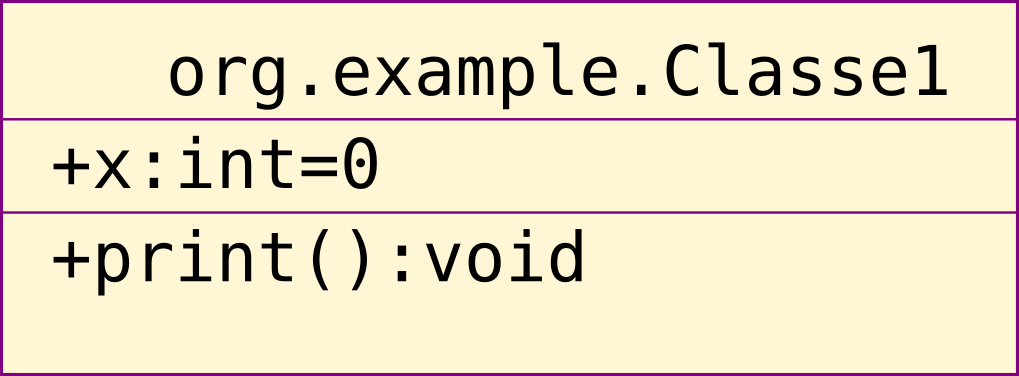
\includegraphics[width=0.5\textwidth]{img/esempio1.png}
  \caption[labelInTOC]{Risultato dell'esportazione del codice dell'esempio 1}
\end{center}
\end{figure}

\subsection{Un esempio un po' più complesso}
In questo secondo esempio viene mostrato come includere il file di modello con
la definizione degli oggetti e si utilizzano alcuni parametri avanzati come:
\begin{itemize}
\item \lstinline{@hide-args} che permette di nascondere i parametri dei metodi
\item \lstinline{@margin} che permette specificare i margini per un gruppo 
nell'ordine \lstinline{top right bottom left} come da standard W3C.
\end{itemize}

\begin{lstlisting}[language=layout, caption={Un esempio un po' più complesso}, style={layout}, label=layout_simple]
import example(*\ref{model_complex}*).u2sm;
[
  @hide-args
  (class org.example.Classe1)
  [
    @margin 0 0 0 300
    (class org.example.Classe2)
  ]
]
\end{lstlisting}

Ecco il risultato dell'esportazione

\begin{figure}[htp]
\begin{center}
  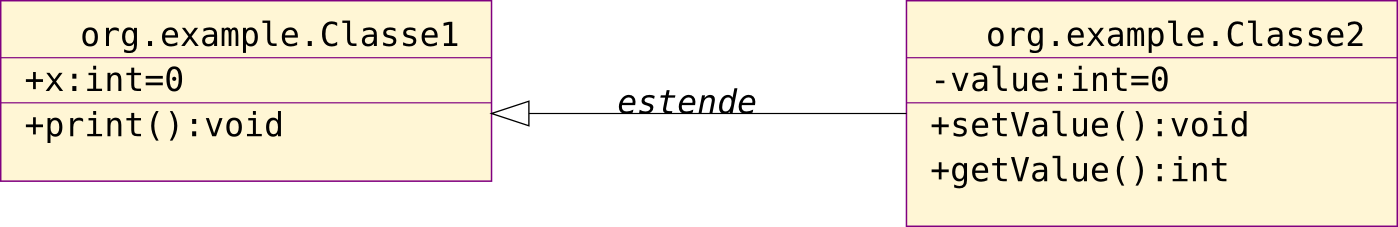
\includegraphics[width=0.9\textwidth]{img/esempio2.png}
  \caption[labelInTOC]{Risultato dell'esportazione del codice dell'esempio 2}
\end{center}
\end{figure}
